\chapter*{Methods}
\label{ch:capitolo2}
The dataset used in this project is a sampled subset of English-language
songs derived from the \textit{Genius Song Lyrics Dataset}\textsuperscript{\cite{geniusdataset}}.
The original dataset contained numerous attributes; the ones considered
relevant for model training are:
\begin{itemize}
    \item \textbf{title:} the song's title;
    
    \item \textbf{lemmatized\_stanzas:} lyrics of the single stanza;
    
    \item \textbf{stanza\_number:} identifies the position of the stanza in the song;

    \item \textbf{is\_chorus:} boolean variable that attests whether the stanza is
        a chorus or not;
    
    \item \textbf{is\_country, is\_pop, is\_rap, is\_rb, is\_rock:} boolean variables, result of a one-hot encoding process, that represent songs genres;

    \item \textbf{label:} represents the emotional classification of the stanza,
        assigned by Albert Base v2\textsuperscript{\cite{albert-base-v2}}.
\end{itemize}
All of these attributes, except for \texttt{title}, were the result
of the preprocessing phase, as described in the preprocessing section.
Due to limited computational power, the labeling process was time-intensive,
ultimately resulting in a limited dataset, with a few more than 100.000 entries.

%PREPROCESSING
\section*{Preprocessing}
\label{preprocessing}
The preprocessing phase began by sampling the dataset while maintaining genre
distribution. Text cleaning focused on removing irrelevant noise, such as
square-bracketed items, and splitting lyrics into individual stanzas using
stanza-related keywords (e.g., "chorus", "verse").
Uninformative stanzas, such as empty or very short ones, were discarded,
resulting in a dataset of numbered stanzas.
A boolean feature, \texttt{is\_chorus}, was added to mark repeated or chorus-related
stanzas, and duplicate stanzas were removed to eliminate redundancy.
Further cleaning involved removing stanza headers and newline characters,
producing cleaner stanzas for labeling.
Lemmatization was performed using the \texttt{spaCy} library, generating
tokenized stanzas by filtering out punctuation. ALBERT Base v2 was then
fine-tuned to label approximately 100,000 stanzas with emotional categories.
A preliminary class distribution analysis showed a slight imbalance, with
\textit{joy} being the most frequent (18\%) and \textit{disgust} the least (10\%).
Figure~\ref{fig:enter-label} illustrates the distribution across all classes.


% The initial preprocessing step involved sampling from the original dataset
% while maintaining the proportional distribution of genres.
% This approach ensured that the genre representation in the sampled subset
% accurately reflected that of the full dataset.\\

% The preliminary text cleaning process focused on the \texttt{lyrics} attribute,
% which contained the complete lyrics of each song in string format.
% Initially, a regular expression (RegEx) was built to remove noise from the
% lyrics, specifically targeting words enclosed in square brackets that were
% irrelevant to the stanza splitting process. Many keywords marking different
% stanzas were written within square brackets, and removing non-keyword items
% inside brackets was crucial to avoid potential issues.\\

% The next critical step was stanza splitting. After cleaning texts from
% noisy square-bracketed items, lyrics were split based on various keywords
% used to denote stanzas (such as "chorus", "verse", "intro", "outro", "refrain", "hook", etc.).
% The RegEx developed accounted for the different formats in which these keywords
% appeared, including square brackets, parentheses, or no brackets at all, as well
% as stanzas separated only by double newline characters.
% The output of this step was, for each song record, a list of strings
% representing individual stanzas (each stanza has also a header with the corresponding
% keyword; this aspect will be discussed in the next paragraph).
% Next, uninformative strings—such as empty strings or those with fewer
% than 20 characters—were removed, as they were too short to provide meaningful
% content.
% As a result, the output of this preliminary preprocessing phase was a dataset
% where the records were no longer whole songs but individual stanzas, each
% numbered according to its position within the song.\\

% A further and more detailed cleaning process on the stanzas involved the creation
% of the boolean feature \texttt{is\_chorus}, which was assigned a \texttt{true}
% value for repeated stanzas within the same song or for stanzas with headers such
% as "hook", "chorus", "refrain", or "bridge".
% Next, stanza headers and newline characters between verses were removed to obtain
% cleaner stanzas.
% Since choruses, hooks, bridges, and refrains often repeat throughout songs,
% duplicate stanzas were discarded to avoid redundant data. This resulted in a
% dataset of cleaned, non-duplicate stanzas, which served as the checkpoint for
% the labeling step and the starting point for the text lemmatization process.\\

% The subsequent step involved lemmatizing the stanzas using the \texttt{spaCy}
% library. A list of lemmatized tokens was created by filtering out punctuation
% and empty words. Lemmatization was chosen over stemming because it produces
% more accurate and meaningful results, particularly for tasks requiring semantic
% understanding, such as the one at hand.\\

% Since the dataset was not pre-labeled at the stanza level, ALBERT Base v2 was employed for this task.
% This transformer model is specifically designed to be fine-tuned on tasks that
% require an understanding of the entire sentence, such as sequence classification. As specified above, due to computational issues the labeling was performed on around 100'000 stanzas. 
% A preliminary analysis of the distribution of the classes revealed a slight disparity in representation among the labels, which is expected in this scenario. 
% The most represented class was \textit{joy}: around 18\% of the total number of texts were classified as such, followed by \textit{fear} and \textit{anger} at 14\% each. 
% The categories \textit{sadness}, \textit{trust}, \textit{anticipation} and \textit{surprise} each constituted 11\%, while \textit{disgust} was the least represented at 10\%. 
% Figure~\ref{fig:enter-label} shows the number of stanzas belonging to each label.
\begin{figure}[H]
    \centering
    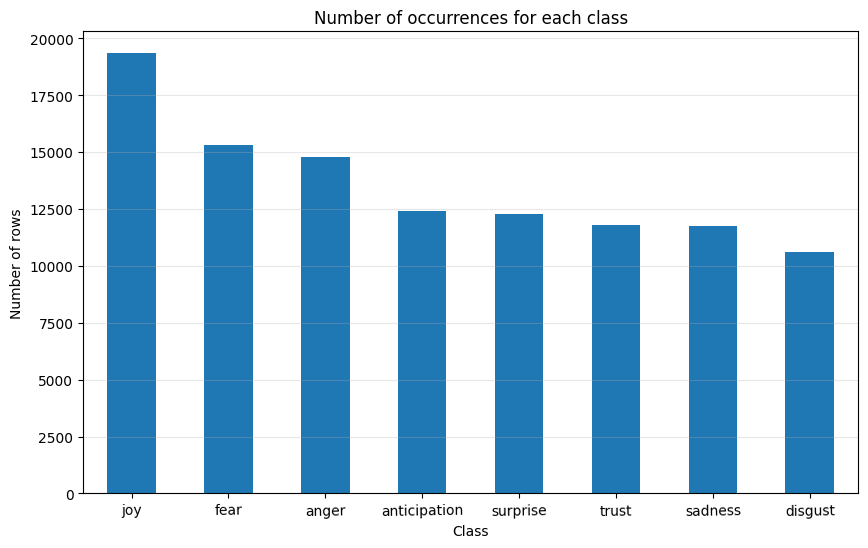
\includegraphics[width=0.7\linewidth]{pictures/exploratory_graph.png}
    \caption{Number of stanzas for each label}
    \label{fig:enter-label}
\end{figure}

\section*{Models}
The selected model architectures are:
\begin{itemize} 
    \item \textbf{Random Forest}: A robust ensemble learning method known for
    its ability to handle complex, high-dimensional datasets effectively.
    \item \textbf{Support Vector Machine (SVM)}: A powerful classifier that
    excels in separating classes by finding the optimal hyperplane,
    particularly effective in text classification tasks.
    \item \textbf{One-Dimensional Convolutional Neural Network (1D-CNN)}:
    Designed to capture local patterns in sequential data, leveraging
    convolutional layers to learn hierarchical features.
    \item \textbf{Recurrent Neural Network (RNN)}: Utilized for its strength
    in processing sequential data, with the ability to capture contextual
    relationships between words across different stanzas.
\end{itemize}
Their different approaches and depths are an important point of the study, as they
offer interesting insights into the possible different techniques and levels of
complexity required for detecting emotional tones in complex pieces of text.

%MODELLI STATICI
\subsection*{Static Models}
% The development of static models was then simple and straight forward.
% Static models are here meant to provide a performance comparison
% for the more complex Neural Networks.
% The two architectures are the same, consisting of a preprocessing
% layer to handle the inputs, followed by the classifier itself.\\

% The preprocessing layers handle both \texttt{title} and
% \texttt{lemmatized\_stanzas} through TF-IDF for feature extraction.
% An additional analysis aimed at identifying the most significant features for
% each emotion label in the dataset was conducted to enhance classification.
% Feature importance analysis was performed on the already labeled and
% lemmatized dataset, following these steps:
% \begin{itemize}
%     \item \textbf{Custom Stopword List Creation}: A custom stopword list was
%     compiled, consisting
%     of the most frequent and generic words in the dataset, along with additional
%     punctuation marks and common typographical errors not covered by the default
%     NLTK stopword lists.

%     \item \textbf{Stopword Removal}: Irrelevant words identified by the custom
%     stopword list were removed from the lemmatized stanzas to reduce noise in
%     the data.

%     \item \textbf{TF-IDF Analysis per Label}: A function was developed to
%     compute TF-IDF scores for a given text, with parameters \texttt{min\_df}
%     set to 2 and \texttt{max\_df} set to 0.80.
% \end{itemize}
% This configuration ensured that words appearing in fewer than two or
% more than 80\% of the documents were ignored, minimizing the influence of
% extremely rare or overly common words. The function was applied separately to
% the cleaned stanzas for each label, with the aim of identifying the most
% relevant features per emotion category.
% The results, however, did not meet expectations, though the outcome was not
% entirely surprising. Most labels shared at least two common features, and
% certain labels (such as surprise and trust) shared all features.
% Additionally, all identified features exhibited very low TF-IDF scores,
% below 0.05.
% This result appears to be inherent to the nature of the dataset: song lyrics
% frequently contain repetitive and generic language, making it difficult to
% distinguish specific emotions based solely on textual features.
% Consequently, the analysis was concluded at this point.\\

% Random Search was chosen for hyperparameter tuning, for both models.
% Cross validation is also used in order to provide a more accurate
% estimate of model performance.
The development of static models aimed at providing a performance benchmark for
more complex neural networks.
Both architectures consisted of a preprocessing layer, followed by a classifier.
The preprocessing handled title and \texttt{lemmatized\_stanzas} using TF-IDF for feature
extraction.\\

To improve classification, feature exctraction was conducted on the labeled dataset. Firstly, we deepened the preprocessing by devising a \textbf{custom stopword list} of frequent and generic words, punctuation, and common typographical errors. To this list were then added the NLTK stopword one and the NLTK numbers' one.
Then, TF-IDF scores were computed for each emotion label, using the parameters \texttt{min\_df} and \texttt{max\_df} to minimize the influence of overly common or rare words. \\
Despite these efforts, the analysis did not yield the expected results, with most labels sharing common features and low TF-IDF scores.
This was likely due to the repetitive and generic nature of song lyrics.\\
With regard to hyperparameters tuning, Random Search and cross-validation were used to
estimate model performance more accurately.



\subsection*{Neural Networks}
% The architectures were developed and tuned through empirical,
% reiterated testing. These parameters helped with the process, and can
% be used for further experimentation.
% Both the Recurrent Neural Network and the One-Dimensional Convolutional
% Neural Network share the same preprocessing
% architecture. Most attributes are processed in the same manner as in
% the Static Models; specific steps are applied to \texttt{lemmatized\_stanzas}
% and \texttt{title}.
% Non-Negative Matrix Factorization is applied to \texttt{title} in addition to
% Term Frequency-Inverse Document Frequency
% to extract latent topics, providing a richer representation of the
% textual data.\\

% \texttt{lemmatized\_stanzas} are handled by Convolutional and Recurrent
% pipelines of the two networks.
% Elements are first tokenized, and then padded in order to
% get an input with consistent shape, which is essential for both types of
% recurrent layers.
The neural network architectures were developed and tuned through empirical
testing. Both the Recurrent
Neural Network and One-Dimensional Convolutional Neural Network share the same
preprocessing steps: Non-Negative Matrix Factorization is applied to title
for extracting latent topics, following TF-IDF for richer text representation.
The \texttt{lemmatized\_stanzas} are processed through convolutional and
recurrent pipelines, where elements are tokenized and padded to maintain
consistent input shapes.

\subsubsection*{One-Dimensional Convolutional Neural Network}
The Convolutional part of the architecture is specifically designed to extract and learn
local patterns in \texttt{embedding\_lyrics}.
Its structure consists of three convolutional layers, each applying filters of
varying sizes. This allows to detect patterns at different granularities.
These layers are followed by Global Max Pooling, to reduce the previous output's
dimension to a fixed-length vector, as well as retaining focus on the most
informative patterns.
A dropout layer is then applied, to introduce regularization and prevent
overfitting.

\subsubsection*{Recurrent Neural Network}
The Recurrent part of the architecture is specifically designed to extract and learn
local patterns in \texttt{embedding\_lyrics}.
Its structure consists of three Gated Recurrent Units (\texttt{GRU} layers)
to model temporal relationships. These are characterized by progressively smaller
numbers of units; this allows pattern capture at different abstraction levels.
All three layers in the architecture use the \texttt{tanh} activation function
to compute the hidden state and
the \texttt{sigmoid} activation function for the recurrent gate.
The first and second layers return the full sequence of hidden states for each
time step in the input sequence, enabling richer learning of patterns over time.
Dropout is applied on every layer, to prevent overfitting and add regularization.

\subsection*{Shared Components}
% The remaining features are handled by a simple pipeline, which concatenates
% their Input layers.
% The inputs are passed them through a dense layer to create a compact
% representation.
% The output of the lyrics-processing branch is concatenated with the processed
% additional features.
% The combined representation is passed through a Dense layer with 32 units
% (ReLU activation), followed by a Dropout layer with a rate of 0.3.
% Finally, the output layer uses 8 units with a softmax activation, corresponding
% to the classification into 8 emotion categories.\\

% The models are trained using categorical cross-entropy as the loss function,
% as it consistently produced better-performing results for both types of
% neural networks.
% As evaluation metric, the better performing one was categorical accuracy.
% Other metrics were tested for evaluation purposes, particularly
% top-k categorical accuracy with $k=2$, which yielded interesting insights
% by considering a prediction correct if the true label is among the top two
% predicted classes. While it showed potential in improving generalization and
% preventing overfitting, it was ultimately discarded as a primary evaluation
% metric. This is because, with $k=2$, the model has a 25\% baseline
% chance of being correct when there are eight possible classes, which reduces
% the precision required for accurate learning and limits performance improvements.\\
Other features are processed through a simple pipeline, which concatenates inputs,
passes them through a dense layer, and combines them with the lyrics-processing
output. The final output layer uses 8 units with softmax activation for emotion
classification.\\

The models are trained using categorical cross-entropy as the loss function, and
categorical accuracy as the evaluation metric. Other metrics, such as top-k
categorical accuracy with $k=2$, were tested but discarded due to limited
performance improvements and lower precision.

% In addition to standard supervised learning, the script supports semi-supervised
% learning. It can be utilized either strictly for transfer learning or in a data
% augmentation approach. When using the data augmentation approach, the model's
% weights can be reset prior to training on the newly pseudo-labeled data, allowing
% for more robust retraining on an expanded dataset.
% The results obtained 